\subsection{CNN - Convolutional Neural Networks}
\label{back:cnn}

\acrfull{cnn}, like the linear layer discussed in section \ref{back:linear}, is a type of feed forward networks commonly used in deep learning. First properly introduced in 1989 \cite{NIPS1989_53c3bce6}, they rely on kernel operations such as a convolution or matrix multiplication to calculate features.    \\

\begin{figure}[h]
    \centering
    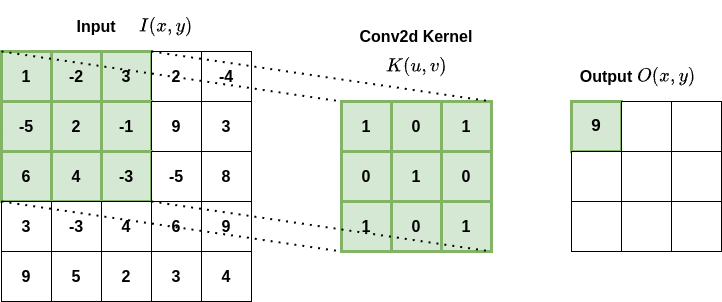
\includegraphics[width=0.8\linewidth]{figures/convolution.png}
    \caption{Example of a 2D Convolution}
    \label{fig:2dconv}
\end{figure}

A convolution is a matematical operation which can be described continiously as such:

\begin{equation}
(f * g)(t) = \int_{-\infty}^{\infty} f(\tau) g(t - \tau) d\tau
\label{eq:contconv}
\end{equation}

\begin{equation}
   (f * g)(x, y) = \sum_{m=0}^{M-1} \sum_{n=0}^{N-1} f(m, n)g(x-m, y-n) 
\label{eq:conv}
\end{equation}

Compared to linear layers, \acrshort{cnn}s are better at extracting more complex features and combating the vanishing gradient problem. Only the size of the kernel is used to stored neurons when performing cross correlation convolution, compared to linear layers where all the weights between layers needs to be stored. These types of networks are highly applicable to numerous different tasks, such as recognition, classification and language model tasks. \\

\subsubsection{Pooling}

Typically, a convolution is followed by an activation function and then a pooling operation. A pooling operation works like a filter $f$, selecting a certain value from a set of numbers based on a measurement. The three most common operations are \textit{max pool}, \textit{min pool} and \textit{avg pool}. Out of these, the \textit{max pool} operation operation is most commonly used. This operation reduces dimensionality, outputting only the most important feature for future layers. \\


\begin{figure}[h]
    \centering
    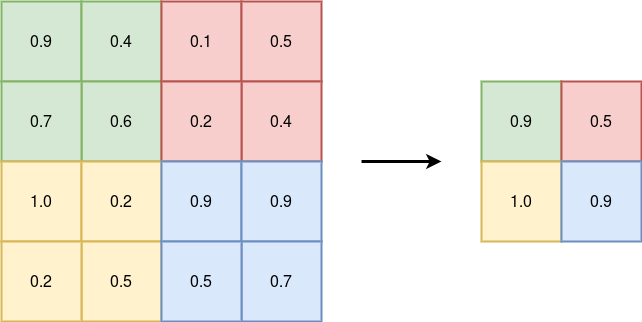
\includegraphics[scale=0.4]{figures/pooling.png}
    \caption{Example of a $2 x 2$ max pool operation with stride 2}
    \label{fig:maxpool}
\end{figure}